
%%% Template originaly created by Karol Kozioł (mail@karol-koziol.net) and modified for ShareLaTeX use

\documentclass[a4paper,11pt]{article}

\usepackage{amsmath}
\usepackage[T1]{fontenc}
\usepackage[utf8]{inputenc}
\usepackage{graphicx}
\usepackage[usenames,dvipsnames]{xcolor}

\usepackage{sansmath}
\renewcommand\familydefault{\sfdefault}
\usepackage{tgheros}

\usepackage{amsmath,amssymb,amsthm,textcomp}
\usepackage{enumerate}
\usepackage{multicol}
\usepackage{tikz}
\usetikzlibrary{graphs,automata,arrows,shapes.misc}

\usepackage{geometry}
\geometry{total={210mm,297mm},
left=25mm,right=25mm,%
bindingoffset=0mm, top=20mm,bottom=20mm}


\linespread{1.3}

\newcommand{\linia}{\rule{\linewidth}{0.5pt}}

% custom theorems if needed
\newtheoremstyle{mytheor}
    {1ex}{1ex}{\normalfont}{0pt}{\scshape}{.}{1ex}
    {{\thmname{#1 }}{\thmnumber{#2}}{\thmnote{ (#3)}}}

\theoremstyle{mytheor}
\newtheorem{defi}{Definition}

% my own titles
\makeatletter
\renewcommand{\maketitle}{
\begin{center}
\vspace{2ex}
{\huge \textsc{\@title}}
\vspace{1ex}
\\
\linia\\
\@author \hfill \@date
\vspace{4ex}
\end{center}
}
\makeatother
%%%

% custom footers and headers
\usepackage{fancyhdr}
\pagestyle{fancy}
\lhead{}
\chead{}
\rhead{}
\lfoot{Automatic~Verification Assignment \#5}
\cfoot{}
\rfoot{Page \thepage}
\renewcommand{\headrulewidth}{0pt}
\renewcommand{\footrulewidth}{0pt}
%

% all section titles centered and bolded
\usepackage{sectsty}
\allsectionsfont{\bfseries\large}
%
% add section label
\renewcommand\thesection{Problem~\arabic{section}:}
\renewcommand\thesubsection{(\alph{subsection})}
%

%%%----------%%%----------%%%----------%%%----------%%%

\begin{document}

\title{Homework Assignment~\#5}

\author{R02943142 Hsieh, Chiao}

\maketitle

\section{B\"uchi Automaton}
Define a B\"uchi automaton (by drawing its transition diagram) for each of the following temporal properties.

\subsection{$p$ holds initially (at position 0) and at every third position (3, 6, etc.).}
Answer.
\smallskip \\
The automaton for the property is as follow. It rejects infinite words where $\neg p$ is at one of the positions that are multiple of 3.
\begin{center}
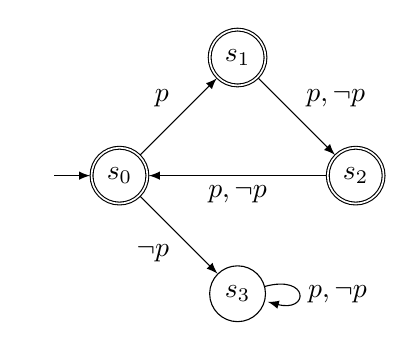
\begin{tikzpicture}
\begin{graph}[circular placement,
  clockwise=4,
  nodes={draw, circle},
  edges={>=latex},
  radius=1.5cm,
  phase=180
  ]{
   "$s_0$"[accepting] <- ""[draw=none],
   "$s_1$"[accepting], 
   "$s_2$"[accepting],
   "$s_3$",
   "$s_0$"->[edge label={$p$}]"$s_1$",
   "$s_0$"->[edge label={$\neg p$}, swap]"$s_3$",
   "$s_1$"->[edge label={$p, \neg p$}]"$s_2$",
   "$s_2$"->[edge label={$p, \neg p$}]"$s_0$",
   "$s_3$"->[edge label={$p, \neg p$}, loop right]"$s_3$"
};
\end{graph}
\end{tikzpicture}
\end{center}

\subsection{Whenever $p$ holds, $q$ must hold eventually at a strictly later position.}
Answer.
\smallskip \\
The automaton for the property is as follow. Basically, it corresponds to the LTL property, $\textbf{AG}(p \rightarrow \textbf{XF} q))$.
\begin{center}
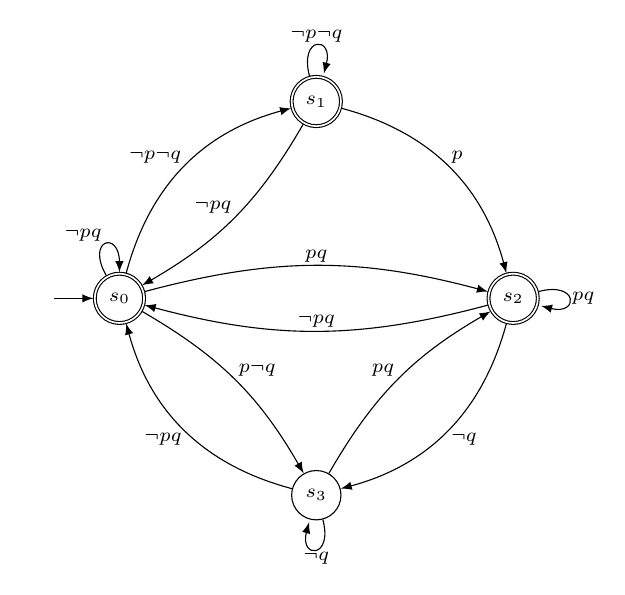
\begin{tikzpicture}[font=\scriptsize]
\begin{graph}[circular placement,
  clockwise=4,
  nodes={draw, circle},
  edges={>=latex, inner sep=1pt},
  radius=2.5cm,
  phase=180
  ]{
   "$s_0$"[accepting] <- ""[draw=none],
   "$s_1$"[accepting], 
   "$s_2$"[accepting],
   "$s_3$",
   "$s_0$"->[edge label={$\neg{p}q$}, out=120,in=90,looseness=8]"$s_0$",
   "$s_0$"->[edge label={$\neg{p}\neg{q}$}, bend left]"$s_1$",
   "$s_0$"->[edge label={$pq$}, bend left=15]"$s_2$",
   "$s_0$"->[edge label={$p\neg{q}$}, bend left=15]"$s_3$",
   "$s_1$"->[edge label={$\neg{p}q$}, bend left=15, swap]"$s_0$",
   "$s_1$"->[edge label={$\neg{p}\neg{q}$}, loop above]"$s_1$",
   "$s_1$"->[edge label={$p$}, bend left]"$s_2$",
   "$s_2$"->[edge label={$\neg{p}q$}, bend left=15, swap]"$s_0$",
   "$s_2$"->[edge label={$pq$}, loop right]"$s_2$",
   "$s_2$"->[edge label={$\neg{q}$}, bend left]"$s_3$",
   "$s_3$"->[edge label={$\neg{p}q$}, bend left]"$s_0$",
   "$s_3$"->[edge label={$pq$}, bend left=15]"$s_2$",
   "$s_3$"->[edge label={$\neg{q}$}, loop below]"$s_3$"
};
\end{graph}
\end{tikzpicture}
\end{center}

\section{LTL to B\"uchi Automata Translation}
Apply the simple on-the-fly translation algorithm to construct a generalized B\"uchi automaton from the LTL formula $(p \land q) \mathcal{U} (p \lor q)$
Please try to illustrate how the algorithm works by showing a few partially constructed automata during the translation.

\noindent Answer.
\smallskip \\
Initially, we begin with the state $s_0$ with the formula $\phi= (p \land q) \mathcal{U} (p \lor q)$.
Following the GPVW algorithm, $s_0$ is split into two states $s_1, s_2$. 
Then, we first process $s_1$ and put $s_2$ into stack. For $s_1$, the $p\land q$ in New is processed,
and two formulae $p$ and $q$ are added to New.
The above steps are shown in the following figure.

\begin{center}
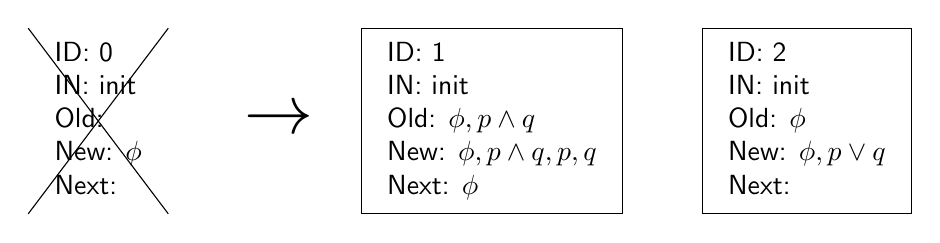
\begin{tikzpicture}[
  every node/.style={draw},
  every edge/.style={>=latex}
  ]
  \node[cross out] (0) at (0, 0){
  \begin{tabular}{l}
    ID: 0 \\
    IN: init \\
    Old: \\
    New: $\phi$ \\
    Next:
  \end{tabular}
  };
  \node (1) at (5,0){
  \begin{tabular}{l}
    ID: 1 \\
    IN: init \\
    Old: $\phi, p \land q$\\
    New: $\phi, p \land q, p, q$ \\
    Next: $\phi$
  \end{tabular}
  };
  \node (2) at (9,0){
  \begin{tabular}{l}
    ID: 2 \\
    IN: init \\
    Old: $\phi$\\
    New: $\phi, p \lor q$ \\
    Next:
  \end{tabular}
  };
  \node[draw=none] (split) at (2.3,0){\Huge $\to$};
\end{tikzpicture}
\end{center}

Next state for $s_1$ is constructed as $s_3$.
$s_3$ is almost identical to $s_0$;
the only difference is that the incoming edge is from $s_1$.
Hence, the state $s_3$ is also split into two states $s_4$ and $s_5$.
$s_4$ is processed and $s_5$ is pushed into stack.
After comparison, $s_4$ is merged with $s_1$. 
Currently, $\{s_2, s_5\}$ are in the stack.

\begin{center}
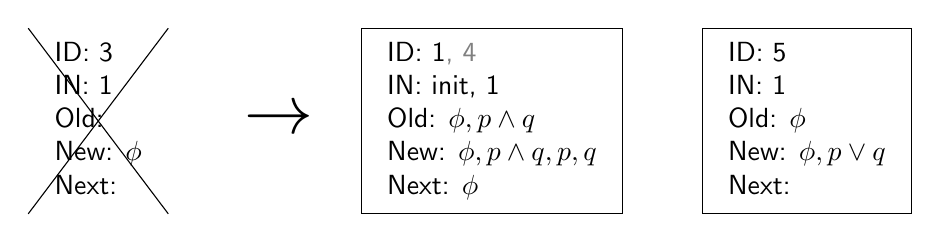
\begin{tikzpicture}[
  every node/.style={draw},
  every edge/.style={>=latex}
  ]
  \node[cross out] (3) at (0, 0){
  \begin{tabular}{l}
    ID: 3 \\
    IN: 1 \\
    Old: \\
    New: $\phi$ \\
    Next:
  \end{tabular}
  };
  \node (1) at (5,0){
  \begin{tabular}{l}
    ID: 1\textcolor{Gray}{, 4} \\
    IN: init, 1 \\
    Old: $\phi, p \land q$\\
    New: $\phi, p \land q, p, q$ \\
    Next: $\phi$
  \end{tabular}
  };
  \node (5) at (9,0){
  \begin{tabular}{l}
    ID: 5 \\
    IN: 1 \\
    Old: $\phi$\\
    New: $\phi, p \lor q$ \\
    Next:
  \end{tabular}
  };
  \node[draw=none] (split) at (2.3,0){\Huge $\to$};
\end{tikzpicture}
\end{center}

Then, we take the last state $s_5$ in the stack.
State $s_5$ is split into two states $s_6$ and $s_7$ due to the formula $p \lor q$.
For $s_6$, since there is no formula in Next, it is processed simply by moving formulae from Old to New and adding a Next state $s_8$ with self loop  and without any formula in Old. 
At this time, $\{s_2, s_7\}$ are in the stack.
$s_7$ is then processed in the same way as $s_6$, and finally only $s_2$ remains in the stack. 

\begin{center}
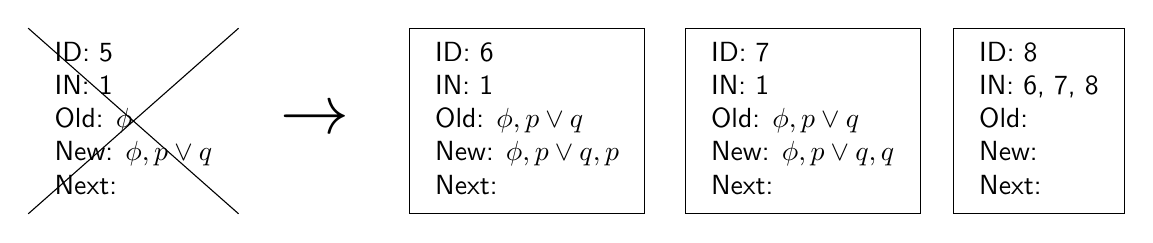
\begin{tikzpicture}[
  every node/.style={draw},
  every edge/.style={>=latex}
  ]
  \node[cross out] (5) at (0, 0){
  \begin{tabular}{l}
    ID: 5 \\
    IN: 1 \\
    Old: $\phi$\\
    New: $\phi, p \lor q$ \\
    Next:
  \end{tabular}
  };
  \node (6) at (5,0){
  \begin{tabular}{l}
    ID: 6 \\
    IN: 1 \\
    Old: $\phi, p \lor q$\\
    New: $\phi, p \lor q, p$\\
    Next:
  \end{tabular}
  };
  \node (7) at (8.5,0){
  \begin{tabular}{l}
    ID: 7 \\
    IN: 1 \\
    Old: $\phi, p \lor q$\\
    New: $\phi, p \lor q, q$\\
    Next:
  \end{tabular}
  };
  \node (8) at (11.5,0){
  \begin{tabular}{l}
    ID: 8 \\
    IN: 6, 7, 8 \\
    Old: \\
    New: \\
    Next:
  \end{tabular}
  };
  \node[draw=none] (split) at (2.3,0){\Huge $\to$};
\end{tikzpicture}
\end{center}

\pagebreak

For $s_2$, it is split into two states $s_9$ and $ s_{10}$ because of 
$p \lor q$. 
However, after checking, $s_9$ is merged with $s_6$ and $s_10$ is merged with $s_7$. 
Therefore, no additional state is introduced.

\begin{center}
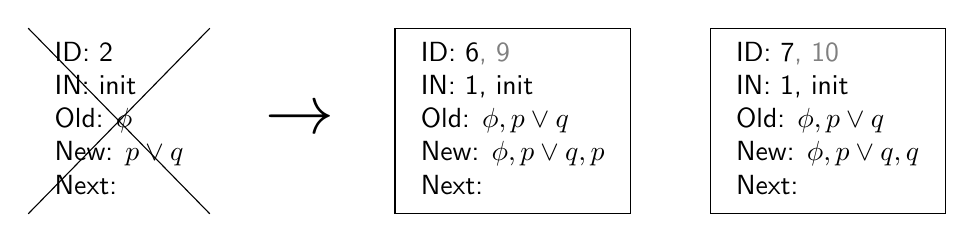
\begin{tikzpicture}[
  every node/.style={draw},
  every edge/.style={>=latex}
  ]
  \node[cross out] (2) at (0, 0){
  \begin{tabular}{l}
    ID: 2 \\
    IN: init \\
    Old: $\phi$\\
    New: $p \lor q$ \\
    Next:
  \end{tabular}
  };
  \node (6) at (5,0){
  \begin{tabular}{l}
    ID: 6\textcolor{Gray}{, 9} \\
    IN: 1, init \\
    Old: $\phi, p \lor q$\\
    New: $\phi, p \lor q, p$\\
    Next:
  \end{tabular}
  };
  \node (7) at (9,0){
  \begin{tabular}{l}
    ID: 7\textcolor{Gray}{, 10} \\
    IN: 1, init \\
    Old: $\phi, p \lor q$\\
    New: $\phi, p \lor q, q$\\
    Next:
  \end{tabular}
  };
  \node[draw=none] (split) at (2.3,0){\Huge $\to$};
\end{tikzpicture}
\end{center}

Now we discuss about the accepting states. There is only one $\mathcal{U}$ operator in $\phi$, so only one set of final state.
The set of states with $p \lor q$ is $\{s_6, s_7\}$, and the set without $\phi$ is $\{s_8\}$. 
Thus, the set of final states is $\{s_6, s_7, s_8\}$.
With the help of GOAL, we then convert the labels on states to labels on edges.
The final automaton should look like below.

\begin{center}
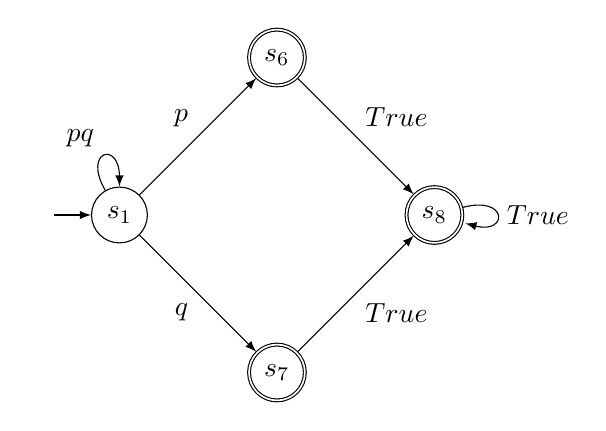
\begin{tikzpicture}
\begin{graph}[circular placement,
  clockwise=4,
  nodes={draw, circle},
  edges={>=latex},
  radius=2cm,
  phase=180
  ]{
   "$s_1$" <- ""[draw=none],
   "$s_6$"[accepting],
   "$s_8$"[accepting],
   "$s_7$"[accepting],
   "$s_1$"->[edge label={$pq$},out=120,in=90,looseness=8]"$s_1$",
   "$s_1$"->[edge label={$p$}]"$s_6$",
   "$s_1$"->[edge label={$q$},swap]"$s_7$",
   "$s_6$"->[edge label={$True$}]"$s_8$",
   "$s_7$"->[edge label={$True$}, swap]"$s_8$",
   "$s_8$"->[edge label={$True$}, loop right]"$s_8$"
};
\end{graph}
\end{tikzpicture}
\end{center}

\end{document}